\chapter{Estado del Arte de Jueces en Línea}
\label{cap:estadoDelArteDeJuecesEnLinea}

\section{Introducción}

Un \textbf{juez en línea} (OJ, del inglés \textit{Online Judge}) es un sistema automatizado accesible vía web que combina un repositorio de problemas de programación con un mecanismo de evaluación automática de soluciones. Los usuarios envían programas que representan propuestas de solución a alguno de los problemas planteados por el sistema. Cada problema define de manera precisa el formato de entrada, la salida esperada y una serie de restricciones que la solución debe cumplir. El juez en línea se encarga de compilar, ejecutar y probar las soluciones enviadas dentro de un entorno controlado y homogéneo, garantizando así condiciones de evaluación justas para todos los participantes, y la seguridad del propio sistema. Su objetivo principal es verificar tanto la corrección como la eficiencia del programa, generando posteriormente un veredicto (\citep{Watanobe_Rahman_Matsumoto_Rage_Ravikumar_2022, Wasik_Antczak_Badura_Laskowski_Sternal_2019}). Entre los veredictos más comunes se encuentran \textit{Accepted} (AC),\textit{Wrong Answer} (WA) o \textit{Time Limit Exceeded} (TLE), aunque la nomenclatura y el conjunto exacto de resultados pueden variar ligeramente entre diferentes sistemas \footnote{Sobre las evaluaciones posibles en Uva Online Judge: \url{https://onlinejudge.org/index.php?Itemid=31&id=16&option=com_content&task=view}}.

\begin{figure}[h]
\centering
\resizebox{\textwidth}{!}{%
\begin{tikzpicture}[
    node distance=1.8cm,
    every node/.style={
        draw,
        rectangle,
        rounded corners,
        align=center,
        minimum width=4.2cm,
        minimum height=1cm
    },
    arrow/.style={->, thick}
]

% Flujo principal
\node (p1) {1. Selección de problema};
\node (p2) [below of=p1] {2. Resolución local};
\node (p3) [below of=p2] {3. Envío de solución};
\node (p4) [below of=p3] {4. Evaluación automatizada};
\node (p5) [below of=p4] {5. Recepción de veredicto};

% Resultado aceptado (sin caja)
\node (ac) [right=3.5cm of p5] {Solución aceptada};

% Flechas principales
\draw[arrow] (p1) -- (p2);
\draw[arrow] (p2) -- (p3);
\draw[arrow] (p3) -- (p4);
\draw[arrow] (p4) -- (p5);

% Veredicto aceptado
\draw[arrow] (p5) -- (ac)
    node[midway, above, draw=none] {AC};

% Iteración (no aceptado)
\draw[arrow]
    (p5.west)
    .. controls +(-4,0) and +(-4,0) ..
    (p2.west)
    node [midway, left, align=center, draw=none]
    {WA, TLE, etc.};

\end{tikzpicture}%
}

\caption{Proceso de uso de un juez en línea y ciclo de iteración}
\label{fig:online-judge-process}
\end{figure}

Los primeros concursos de programación se remontan a la década de 1970 y fueron creciendo progresivamente en popularidad, lo que generó la necesidad de contar con sistemas capaces de evaluar automáticamente grandes volúmenes de código de forma rápida y objetiva. Esta necesidad se hizo especialmente evidente en el contexto de competiciones como la ICPC (International Collegiate Programming Contest), donde la corrección manual de soluciones resultaba inviable. En este escenario comenzaron a desarrollarse los primeros jueces en línea. Uno de los primeros OJs en alcanzar una popularidad global fue UVa Online Judge, creado por el profesor Miguel Ángel Revilla en la Universidad de Valladolid, y hecho disponible al público en general en 1997 (\cite{Revilla_Manzoor_Liu_2008}). Desde entonces, estos sistemas han experimentado un crecimiento notable tanto en número de usuarios como en la cantidad de soluciones enviadas y problemas disponibles \footnote{Estadísticas de uso en Uva Online Judge desde 1997: \url{https://onlinejudge.org/index.php?option=com_onlinejudge&Itemid=23}}.

El uso de los jueces en línea se ha extendido además a múltiples ámbitos más allá de la programación competitiva. Ya en 1961, la Universidad de Stanford utilizaba un sistema automático para evaluar los programas en ALGOL desarrollados por sus estudiantes (\cite{Forsythe_Wirth_1965}). En la actualidad existen numerosos jueces en línea con un enfoque educativo, como CheckiO \footnote{\url{https://checkio.org/}}, Codecademy \footnote{\url{https://www.codecademy.com/}} o Jutge.org \footnote{\url{https://jutge.org/}}, que permiten a los usuarios aprender y practicar conceptos de programación y algoritmia tanto de forma individual como colectiva, por ejemplo en asignaturas universitarias o cursos especializados. Asimismo, los jueces en línea son ampliamente utilizados en procesos de reclutamiento laboral, donde se analizan las soluciones de los candidatos para evaluar sus habilidades técnicas, o como herramienta de preparación para entrevistas. Dos de los OJs más populares dentro de este ámbito son HackerRank, con más de 26,5 millones de desarrolladores registrados \footnote{\url{https://www.hackerrank.com/about-us}}, y LeetCode \footnote{\url{https://leetcode.com/}}.

\section{Categorización de jueces de programación}

Los jueces en línea pueden clasificarse en cuatro categorías principales en función del propósito para el que fueron diseñados. Esta clasificación permite comprender mejor las diferencias en sus objetivos, funcionalidades y público objetivo, así como el tipo de problemas y métricas de evaluación que emplean (\cite{Wasik_Antczak_Badura_Laskowski_Sternal_2019}).

 \begin{enumerate}
     \item \textbf{Jueces de programación competitiva}: Los jueces de programación competitiva están orientados principalmente a la organización y desarrollo de competiciones de programación, tanto a nivel local como internacional. Estos sistemas suelen ofrecer rankings globales o regionales, sistemas de puntuación y límites estrictos de tiempo y memoria, ya que la eficiencia de las soluciones es un aspecto central. Los problemas están diseñados para poner a prueba la capacidad de los participantes en algoritmia, estructuras de datos y optimización, y el énfasis recae en comparar el rendimiento de los usuarios bajo condiciones homogéneas.
     \item \textbf{Jueces educativos}: Los jueces educativos tienen como objetivo principal apoyar el aprendizaje de la programación. En este caso, el énfasis no se encuentra en la competición, sino en el proceso formativo. Estos sistemas suelen integrarse en contextos académicos o de autoaprendizaje, permitiendo a los usuarios practicar conceptos de programación de forma progresiva. La retroalimentación inmediata que ofrecen facilita la detección de errores y la mejora continua, siendo comunes en asignaturas universitarias, cursos especializados o plataformas de aprendizaje en línea.
     \item \textbf{Jueces de reclutamiento}: Los jueces de reclutamiento están diseñados para evaluar las habilidades técnicas de candidatos en procesos de selección de personal. En este contexto, los problemas planteados buscan medir la capacidad del aspirante para resolver tareas concretas de programación dentro de un tiempo limitado. El OJ actúa como una herramienta objetiva que permite comparar soluciones y analizar el desempeño de los candidatos, además de servir como medio de preparación para entrevistas técnicas.
     \item \textbf{Otros jueces}: Finalmente, existen otros jueces en línea orientados a nichos o dominios específicos. Estos sistemas se centran en áreas concretas de la programación o en tecnologías particulares, como puede ser la programación concurrente, el manejo de bases de datos o lenguajes específicos. Aunque su público suele ser más reducido, cumplen un papel importante al cubrir necesidades especializadas que no siempre están contempladas en los jueces generalistas.
 \end{enumerate}

\section{Gamificación}

Uno de los elementos de los jueces en línea modernos de especial interés para el tema de este trabajo es la gamificación. 

La gamificación es una tendencia creciente en los jueces en línea, que busca motivar y fidelizar a los usuarios mediante la incorporación de elementos y mecánicas propias de los juegos (\textit{games} en inglés). El proceso de gamificación no consiste en convertir la plataforma en un juego, sino en enriquecer la experiencia de usuario y aumentar su participación mediante el uso de mecánicas nuevas y la creación de una fuente de motivación extrínseca.
Para que la gamificación sea eficaz, debe integrarse de forma coherente con los objetivos del sistema y el comportamiento deseado en los usuarios (\cite{Zichermann_Cunningham_2011}).

Los mecanismos de gamificación pueden variar según la categoría del juez, ya que cada tipo persigue objetivos diferentes:

\begin{enumerate}
    \item \textbf{Jueces de programación competitiva}: En estas plataformas, la gamificación se centra en la comparación entre usuarios. Se utilizan tablas de clasificación y sistemas de puntuación, que permiten medir el progreso relativo de cada participante y fomentar la competencia. Por ejemplo, Codeforces implementa un sistema de \textit{rating} basado en la participación en concursos, ayudando a los usuarios a identificar su posición dentro de la comunidad y a fijarse objetivos de mejora \footnote{Sobre cómo Codeforces calcula la puntuación de usuario: \url{https://codeforces.com/blog/entry/102}}.
\begin{figure}
    \centering
    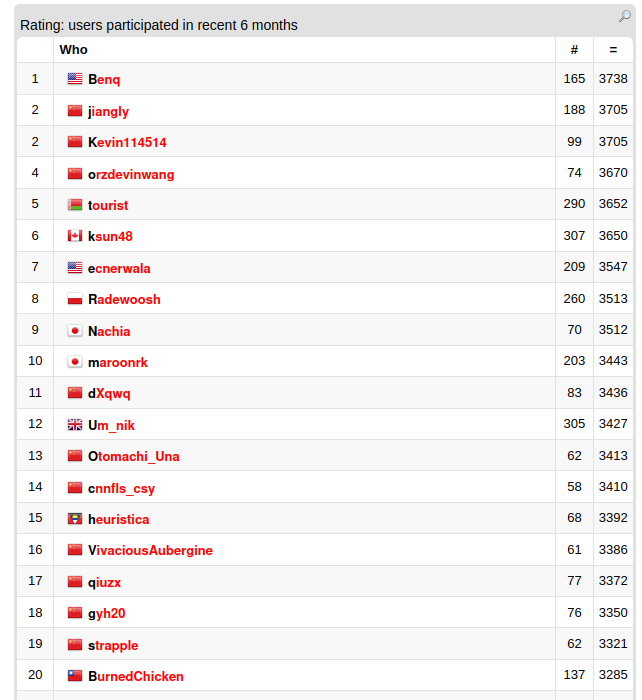
\includegraphics[width=0.6\linewidth]{Imagenes//Bitmap/Leaderboard Codeforces.png}
    \caption{Captura de la tabla de clasificación global de Codeforces}
    \label{fig:Captura de la tabla de clasificación global de Codeforces}
\end{figure}

    \item  \textbf{Jueces educativos}: Estos sistemas aplican la gamificación para reforzar el aprendizaje individual y mantener la motivación del estudiante. Es habitual el uso de insignias (\textit{badges}) y logros, que recompensan tanto la resolución de ejercicios como la constancia y el uso de diferentes lenguajes de programación. Plataformas como HackerRank emplean estas insignias visuales para ayudar al usuario a establecer metas y guiarle a alcanzarlas \footnote{\url{https://www.hackerrank.com/scoring/badges-and-medals}}.
\begin{figure}
    \centering
    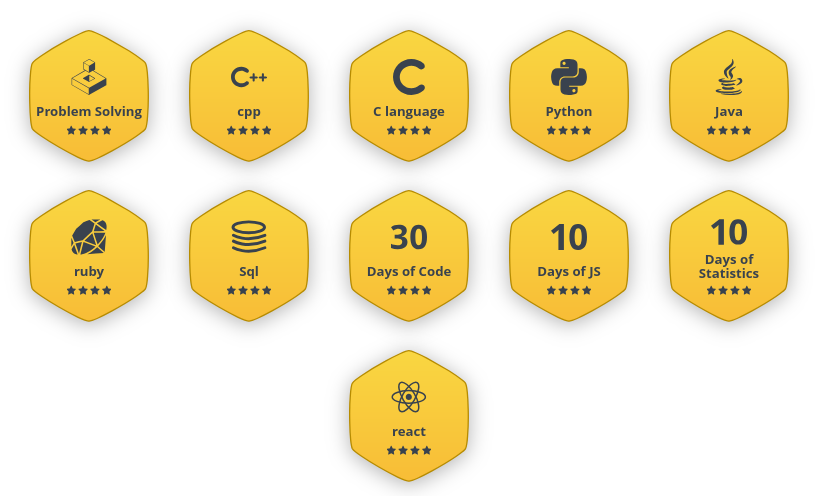
\includegraphics[width=0.6\linewidth]{Imagenes//Bitmap/Badges HackerRank.png}
    \caption{Insignias disponibles en HackerRank}
    \label{fig:Insignias disponibles en HackerRank}
\end{figure}

    \item \textbf{Jueces de reclutamiento}: En este caso, la gamificación está dirigida tanto a demostrar habilidades y conocimientos ante potenciales empleadores como a la preparación para entrevistas técnicas. Aquí, las insignias y logros pueden actuar como una señal visible de competencia técnica. Además, debido al enfoque individualista tanto de los jueces de reclutamiento como de los educativos, las estadísticas se centran en mostrar el propio progreso y mejora del usuario.
\end{enumerate}

\begin{figure}
    \centering
    \includegraphics[width=0.8\linewidth]{Imagenes//Bitmap/Estadísticas Leetcode.png}
    \caption{Estadísticas de Leetcode}
    \label{fig:Estadísticas en Leetcode}
\end{figure}

El OJ \aer ya incluye varias herramientas de gamificación orientadas a seguimiento del progreso individual \footnote{\url{https://aceptaelreto.com/}}. En la pestaña de perfil se muestran estadísticas como:

\begin{itemize}
    \item Cantidad de envíos realizados
    \item Cantidad de envíos correctos
    \item Cantidad de envíos intentados
    \item Cantidad de ejercicios resueltos
    \item Lenguajes más utilizados
    \item Veredictos más recibidos
\end{itemize}

\begin{figure}
    \centering
    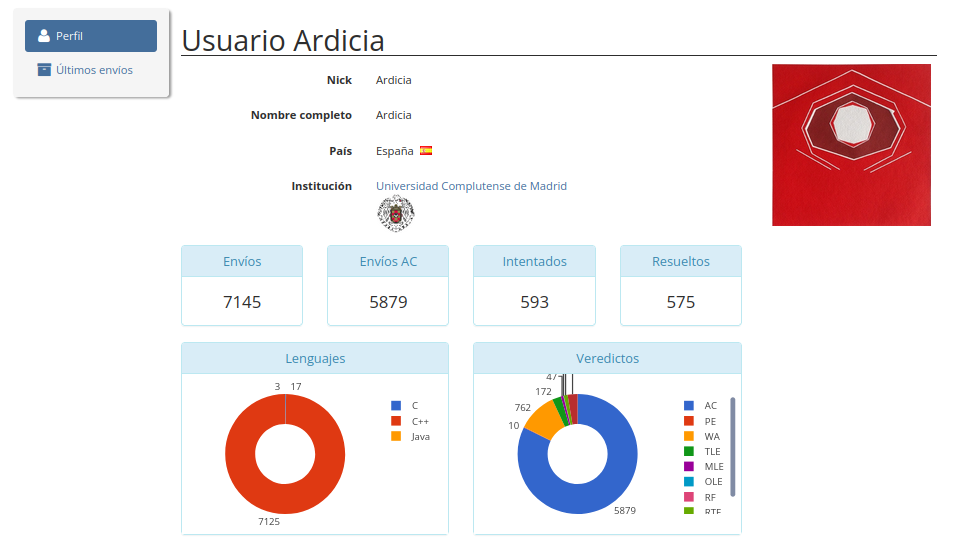
\includegraphics[width=0.8\linewidth]{Imagenes//Bitmap/Estadísticas Acepta el Reto.png}
    \caption{Estadísticas de \aer}
    \label{fig:Estadísticas de Acepta el Reto}
\end{figure}

Estas métricas permiten a los usuarios analizar su evolución y focalizar sus esfuerzos en mejorar áreas concretas, lo cual es coherente con su propósito educativo. Además, la plataforma cuenta con una pestaña de estadísticas que muestra las últimas submissions \footnote{\url{https://aceptaelreto.com/statistics/submissions.php}}.

\begin{table}[h!]
\centering
\small
\begin{tabularx}{\textwidth}{l l X}
\toprule
\textbf{Categoría} & \textbf{Objetivo principal} & \textbf{Elementos de gamificación más comunes} \\
\midrule
Programación competitiva & Rendimiento & Puntuación, tablas de clasificación. \\
Educativo & Aprendizaje & Insignias, logros y estadísticas de progreso. \\
Reclutamiento & Mejorar habilidades & Insignias, logros y estadísticas de progreso. \\
\bottomrule
\end{tabularx}
\caption{Resumen de categorías de jueces en línea y sus elementos de gamificación}
\end{table}

\section{Diseño y arquitectura}

Aunque este trabajo no profundiza en la arquitectura interna de evaluación de los jueces en línea, resulta relevante comprender su estructura como aplicación web y los elementos que la distinguen de otros sistemas web convencionales.

A alto nivel, un juez en línea se compone de dos componentes principales. En primer lugar, se encuentra la parte web, que incluye la interfaz de usuario (\textit{frontend}), el servidor (\textit{backend}) y la base de datos. Esta sección gestiona la interacción del usuario con la plataforma, permitiendo visualizar y seleccionar problemas, enviar código para su evaluación y consultar tanto estadísticas como resultados de sus envíos. La base de datos almacena la información necesaria para mantener un registro de los problemas disponibles, los envíos realizados y los datos de los usuarios.

En segundo lugar, y lo que realmente diferencia a un juez en línea de otras aplicaciones web, se encuentra el sistema de evaluación de código. Este subsistema permite recibir, ejecutar y evaluar código arbitrario enviado por los usuarios, una operación que en cualquier otra plataforma web constituiría un riesgo significativo de seguridad. Para ello, se utilizan demonios de evaluación que monitorizan continuamente los envíos y los ejecutan en entornos seguros y aislados, tales como contenedores, sandboxes o máquinas virtuales (\cite{Kuo_Wen_Hsieh_Huang_2023}). La evaluación se realiza de manera asíncrona, de modo que el usuario puede continuar navegando por la plataforma mientras su envío es procesado. Una vez completada la evaluación, el veredicto se transmite a la parte web, que se encarga de mostrarlo al usuario.

Esta arquitectura permite separar de manera clara las funciones interactivas de la plataforma de las funciones de evaluación de código, garantizando tanto la usabilidad como la seguridad. La capacidad de ejecutar de forma segura código arbitrario constituye la preocupación central de estos sistemas y determina su diseño arquitectónico distintivo.

En síntesis, un juez en línea integra la infraestructura de una aplicación web tradicional con un subsistema especializado para la ejecución segura y asíncrona de código, lo que posibilita ofrecer una plataforma interactiva, confiable y segura para la resolución de problemas de programación.

\section{Conclusiones}

El análisis del estado del arte muestra que la visualización de estadísticas y la gamificación constituyen componentes fundamentales en los jueces en línea modernos, especialmente en aquellos con fines educativos y de reclutamiento. La presentación clara de métricas como envíos correctos, problemas resueltos, veredictos obtenidos y logros alcanzados permite a los usuarios evaluar su progreso, identificar áreas de mejora y mantener la motivación a lo largo del tiempo. Esta funcionalidad depende directamente de la arquitectura del juez, que separa la interfaz web de los subsistemas de evaluación de código, permitiendo actualizar los datos de manera segura y asíncrona. Por tanto, la creación de pantallas de estadísticas y logros no solo mejora la experiencia del usuario, sino que constituye un elemento esencial para el aprendizaje, la constancia y la participación activa en la plataforma.